% GNUPLOT: LaTeX picture with Postscript
\begingroup
  \fontfamily{phv}%
  \selectfont
  \makeatletter
  \providecommand\color[2][]{%
    \GenericError{(gnuplot) \space\space\space\@spaces}{%
      Package color not loaded in conjunction with
      terminal option `colourtext'%
    }{See the gnuplot documentation for explanation.%
    }{Either use 'blacktext' in gnuplot or load the package
      color.sty in LaTeX.}%
    \renewcommand\color[2][]{}%
  }%
  \providecommand\includegraphics[2][]{%
    \GenericError{(gnuplot) \space\space\space\@spaces}{%
      Package graphicx or graphics not loaded%
    }{See the gnuplot documentation for explanation.%
    }{The gnuplot epslatex terminal needs graphicx.sty or graphics.sty.}%
    \renewcommand\includegraphics[2][]{}%
  }%
  \providecommand\rotatebox[2]{#2}%
  \@ifundefined{ifGPcolor}{%
    \newif\ifGPcolor
    \GPcolortrue
  }{}%
  \@ifundefined{ifGPblacktext}{%
    \newif\ifGPblacktext
    \GPblacktextfalse
  }{}%
  % define a \g@addto@macro without @ in the name:
  \let\gplgaddtomacro\g@addto@macro
  % define empty templates for all commands taking text:
  \gdef\gplbacktext{}%
  \gdef\gplfronttext{}%
  \makeatother
  \ifGPblacktext
    % no textcolor at all
    \def\colorrgb#1{}%
    \def\colorgray#1{}%
  \else
    % gray or color?
    \ifGPcolor
      \def\colorrgb#1{\color[rgb]{#1}}%
      \def\colorgray#1{\color[gray]{#1}}%
      \expandafter\def\csname LTw\endcsname{\color{white}}%
      \expandafter\def\csname LTb\endcsname{\color{black}}%
      \expandafter\def\csname LTa\endcsname{\color{black}}%
      \expandafter\def\csname LT0\endcsname{\color[rgb]{1,0,0}}%
      \expandafter\def\csname LT1\endcsname{\color[rgb]{0,1,0}}%
      \expandafter\def\csname LT2\endcsname{\color[rgb]{0,0,1}}%
      \expandafter\def\csname LT3\endcsname{\color[rgb]{1,0,1}}%
      \expandafter\def\csname LT4\endcsname{\color[rgb]{0,1,1}}%
      \expandafter\def\csname LT5\endcsname{\color[rgb]{1,1,0}}%
      \expandafter\def\csname LT6\endcsname{\color[rgb]{0,0,0}}%
      \expandafter\def\csname LT7\endcsname{\color[rgb]{1,0.3,0}}%
      \expandafter\def\csname LT8\endcsname{\color[rgb]{0.5,0.5,0.5}}%
    \else
      % gray
      \def\colorrgb#1{\color{black}}%
      \def\colorgray#1{\color[gray]{#1}}%
      \expandafter\def\csname LTw\endcsname{\color{white}}%
      \expandafter\def\csname LTb\endcsname{\color{black}}%
      \expandafter\def\csname LTa\endcsname{\color{black}}%
      \expandafter\def\csname LT0\endcsname{\color{black}}%
      \expandafter\def\csname LT1\endcsname{\color{black}}%
      \expandafter\def\csname LT2\endcsname{\color{black}}%
      \expandafter\def\csname LT3\endcsname{\color{black}}%
      \expandafter\def\csname LT4\endcsname{\color{black}}%
      \expandafter\def\csname LT5\endcsname{\color{black}}%
      \expandafter\def\csname LT6\endcsname{\color{black}}%
      \expandafter\def\csname LT7\endcsname{\color{black}}%
      \expandafter\def\csname LT8\endcsname{\color{black}}%
    \fi
  \fi
  \setlength{\unitlength}{0.0500bp}%
  \begin{picture}(5760.00,2520.00)%
    \gplgaddtomacro\gplbacktext{%
      \csname LTb\endcsname%
      \put(918,540){\makebox(0,0)[r]{\strut{} 0}}%
      \csname LTb\endcsname%
      \put(918,720){\makebox(0,0)[r]{\strut{} 0.01}}%
      \csname LTb\endcsname%
      \put(918,900){\makebox(0,0)[r]{\strut{} 0.02}}%
      \csname LTb\endcsname%
      \put(918,1080){\makebox(0,0)[r]{\strut{} 0.03}}%
      \csname LTb\endcsname%
      \put(918,1260){\makebox(0,0)[r]{\strut{} 0.04}}%
      \csname LTb\endcsname%
      \put(918,1440){\makebox(0,0)[r]{\strut{} 0.05}}%
      \csname LTb\endcsname%
      \put(918,1620){\makebox(0,0)[r]{\strut{} 0.06}}%
      \csname LTb\endcsname%
      \put(918,1800){\makebox(0,0)[r]{\strut{} 0.07}}%
      \csname LTb\endcsname%
      \put(918,1980){\makebox(0,0)[r]{\strut{} 0.08}}%
      \csname LTb\endcsname%
      \put(1026,360){\makebox(0,0){\strut{} 0}}%
      \csname LTb\endcsname%
      \put(1764,360){\makebox(0,0){\strut{} 0.005}}%
      \csname LTb\endcsname%
      \put(2502,360){\makebox(0,0){\strut{} 0.01}}%
      \csname LTb\endcsname%
      \put(3240,360){\makebox(0,0){\strut{} 0.015}}%
      \csname LTb\endcsname%
      \put(3978,360){\makebox(0,0){\strut{} 0.02}}%
      \csname LTb\endcsname%
      \put(4716,360){\makebox(0,0){\strut{} 0.025}}%
      \csname LTb\endcsname%
      \put(5454,360){\makebox(0,0){\strut{} 0.03}}%
      \put(180,1260){\rotatebox{90}{\makebox(0,0){\strut{}FRR}}}%
      \put(3240,90){\makebox(0,0){\strut{}FAR}}%
      \put(3240,2250){\makebox(0,0){\strut{}UND: Recognition Performance}}%
    }%
    \gplgaddtomacro\gplfronttext{%
      \csname LTb\endcsname%
      \put(4635,1827){\makebox(0,0)[r]{\strut{}neutral model}}%
      \csname LTb\endcsname%
      \put(4635,1647){\makebox(0,0)[r]{\strut{}expression model}}%
    }%
    \gplbacktext
    \put(0,0){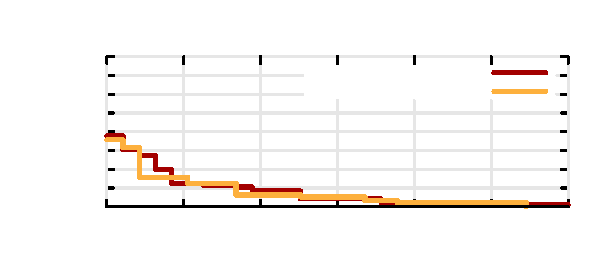
\includegraphics{und_FARFRR}}%
    \gplfronttext
  \end{picture}%
\endgroup
